\chapter{實驗結果與分析}
\label{cha:Evaluation}

此章節中,我們將針對前述第~\ref{cha:Method}~章之研究方法進行實驗結果評估與分析,其中包含:第~\ref{sec:SystemStructure}~節\ 實驗系統架構、第~\ref{sec:DataPreprocessEvaluation}~節\ 資料前處理評估、第~\ref{sec:DataAnalysisEvaluation}~節\ 資料分析評估、第~\ref{sec:MachineLearningEvaluation}~節\ 機器學習評估以及第~\ref{sec:PredictionResultAnalysisEvaluation}~節\ 預測結果分析評估。

\section{實驗系統架構}
\label{sec:SystemStructure}

本論文實驗系統架構將分為資料前處理端、資料分析端與機器學習端,如表~\ref{tab:ResearchEnvironment},並均以\emph{Python}做為開發語言。

\begin{itemize}
    \item [■] 資料前處理端:以\emph{Apache Spark}~\cite{armbrust2015spark}處理資料之前處理以及分割資料集所使用。
    \item [■] 資料分析端:以\emph{missingno}~\cite{Bilogur2018}、\emph{Seaborn}~\cite{michael_waskom_2020_3767070}協助以圖表方式呈現資料特性。
    \item [■] 機器學習端:以\emph{pandas}~\cite{jeff_reback_2020_3715232}~\cite{mckinney-proc-scipy-2010}、\emph{scikit-learn}~\cite{scikit-learn}~\cite{sklearn_api}、\emph{XGBoost}~\cite{chen2016xgboost}處理機器學習訓練與評估。
\end{itemize}

\begin{table}[!htb]
	\centering
	\begin{tabular}{cclclcl}
	\hline \hline
	系統端點 && 資料前處理端 && 資料分析端 && 機器學習端 \\
    \hline \hline
    \multirow{3}*{研究環境} && \emph{Apache Spark} && \emph{missingno} && \emph{pandas} \\
    &&&& \emph{Seaborn} && \emph{scikit-learn} \\
    &&&&&& \emph{XGBoost} \\
    \hline \hline
	\end{tabular}
	\caption[實驗系統架構之研究環境表]{實驗系統架構之研究環境表}
	\label{tab:ResearchEnvironment}
\end{table}

我們所使用之資料集包含1,824,962位玩家及其遊戲行為軌跡,總容量約為12.2 GB。
\newpage

\section{資料前處理評估}
\label{sec:DataPreprocessEvaluation}

此階段將評估前章 \ref{subsubsec:MissingValueHandle}~小節之資料空缺值處理、\ref{subsubsec:NonValuePlayerHandle}~小節之無價值玩家處理以及兩小節~\ref{subsec:ClassPreparation} 及 \ref{subsec:FeatureMining} 之目標值與資料特徵處理,分別於 \ref{subsec:CleanDataEvaluation}~小節\ 清理資料評估及 \ref{subsec:ClassAndFeatureEvaluation}~小節\ 目標值與資料特徵評估說明。

\subsection{清理資料評估}
\label{subsec:CleanDataEvaluation}

我們將從玩家資料中刪除有空缺值存在之玩家,並再刪除該玩家之遊戲行為軌跡,如圖~\ref{fig:eva_MissingValueHandle},透過\emph{missingno}產出圖表,Country為設備所在地、DeviceName為設備型號、DeviceBrand為設備廠牌、Platform為設備平台,可以從圖中看出,僅有設備廠牌存在空缺值,共有18,037位玩家,另外除了有空缺值存在外,還有值為「Unknown」之資料,將同樣視為空缺值予以刪除,共有10,198位玩家。共刪除28,235位玩家,約占總玩家1.55 \%。

\begin{figure}[!htb]
    \begin{center}
      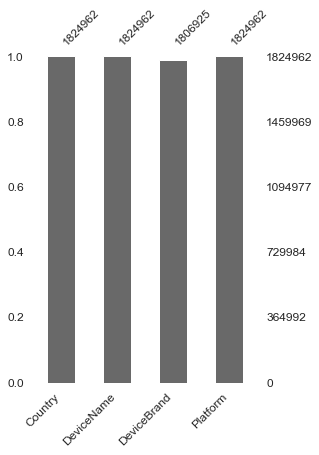
\includegraphics[width=0.5\textwidth]{figures/evaluation/Image_MissingValueHandle.png}
      \caption[玩家資料空缺值示意圖]{玩家資料空缺值示意圖\ (\ X軸為玩家資料之資料特徵名;Y軸為該資料特徵非空缺值樣本數量\ )\ }
      \label{fig:eva_MissingValueHandle}
    \end{center}
\end{figure}
\newpage

我們將從各項遊戲原始資料集中撈取$N$天 ( 無價值玩家觀察期\ ) 內的遊戲行為軌跡,並於$N$值代入1,\ 2,\ 3,\ 4,\ 5,分別代表觀察1,\ 2,\ 3,\ 4,\ 5天內之玩家是否有遊玩過各項遊戲,實驗結果如表~\ref{tab:NonValuePlayerObservation}。

\begin{table}[!htb]
	\centering
	\begin{tabular}{ccrcr}
	\hline \hline
	無價值玩家觀察期 && 無價值玩家數 && 無價值玩家佔比 \\
    \hline \hline
    $N = 1$ && 331,207 && 18.43 \% \\
    \hline
    $N = 2$ && 305,058 && 16.98 \% \\
    \hline
    $N = 3$ && 299,314 && 16.66 \% \\
    \hline
    $N = 4$ && 295,826 && 16.46 \% \\
    \hline
    $N = 5$ && 293,108 && 16.31 \% \\
    \hline \hline
	\end{tabular}
	\caption[無價值玩家觀察表]{無價值玩家觀察表}
	\label{tab:NonValuePlayerObservation}
\end{table}

有價值玩家數將由玩家總數扣除空缺值玩家數與無價值玩家數,如表~\ref{tab:ValuePlayerObservation},從表中可以看出,$N$值於1至5間之有價值玩家數差距不大,約在1,500,000位左右。本論文將挑選$N = 3$做後續實驗,即為1,497,413位有價值玩家。

\begin{table}[!htb]
	\centering
	\begin{tabular}{cccrr}
	\hline \hline
	玩家總數 & 空缺值玩家數 & 無價值玩家觀察期 & 無價值玩家數 & 有價值玩家數 \\
    \hline \hline
    \multirow{5}*{1,824,962} & \multirow{5}*{28,235} & $N = 1$ & 331,207 & 1,465,520 \\
    \cline{3-5}
    && $N = 2$ & 305,058 & 1,491,669 \\
    \cline{3-5}
    && \cellcolor[HTML]{C0C0C0}$N = 3$ & \cellcolor[HTML]{C0C0C0}299,314 & \cellcolor[HTML]{C0C0C0}1,497,413 \\
    \cline{3-5}
    && $N = 4$ & 295,826 & 1,500,901 \\
    \cline{3-5}
    && $N = 5$ & 293,108 & 1,503,619 \\
    \hline
    \multicolumn{5}{c}{有價值玩家數 $=$ 玩家總數 $-$ 空缺值玩家數 $-$ 無價值玩家數} \\
    \hline \hline
	\end{tabular}
	\caption[有價值玩家觀察表]{有價值玩家觀察表}
	\label{tab:ValuePlayerObservation}
\end{table}
\newpage

\subsection{目標值與資料特徵評估}
\label{subsec:ClassAndFeatureEvaluation}

我們將從玩家資料與玩家消費紀錄中定義$M$天\ (\ 付費玩家定義期\ )\ 內有消費行為之玩家,並且$M$值最小值必須不小於$N$值,即為3天,故$M$值代入3,\ 4,\ 5,\ 6,\ 7,分別代表觀察3,\ 4,\ 5,\ 6,\ 7天內之玩家是否有消費行為,如表~\ref{tab:PayerAndNonPayerDefinition},本論文將挑選$M = 7$做後續實驗,即為41,584位付費玩家及1,455,829位非付費玩家。

\begin{table}[!htb]
	\centering
	\begin{tabular}{crrrr}
	\hline \hline
	付費玩家定義期 & 付費玩家數 & 付費玩家佔比 & 非付費玩家 & 非付費玩家佔比 \\
    \hline \hline
    $M = 3$ & 35,088 & 2.43 \% & 1,462,325 & 97.57 \% \\
    \hline
    $M = 4$ & 37,504 & 2.50 \% & 1,459,909 & 97.50 \% \\
    \hline
    $M = 5$ & 39,137 & 2.61 \% & 1,458,276 & 97.39 \% \\
    \hline
    $M = 6$ & 40,425 & 2.70 \% & 1,456,988 & 97.30 \% \\
    \hline
    \rowcolor[HTML]{C0C0C0}
    $M = 7$ & 41,584 & 2.78 \% & 1,455,829 & 97.22 \% \\
    \hline \hline
	\end{tabular}
	\caption[付費玩家及非付費玩家定義表]{付費玩家及非付費玩家定義表}
	\label{tab:PayerAndNonPayerDefinition}
\end{table}

定義一消費速度,即為將付費日 $-$ 創立帳號日,透過\emph{Seaborn}產出圖表,圖~\ref{fig:eva_PlayerConsumePeriod} 為觀察付費玩家之消費速度,從圖中可以看出,玩家於創立帳號日當天即消費者為多數,隨著天數增加,消費意願則降低;故本論文將聚焦於新進之潛在玩家,以保握住玩家高消費意願時期。

\begin{figure}[!htb]
    \begin{center}
      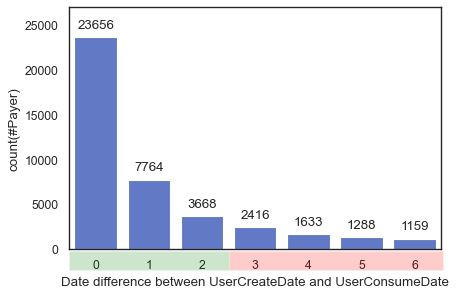
\includegraphics[width=0.7\textwidth]{figures/evaluation/Image_PlayerConsumePeriod.png}
      \caption[付費玩家之消費速度圖]{付費玩家之消費速度圖 ( X軸為付費玩家之消費速度;Y軸為付費玩家數 ) }
      \label{fig:eva_PlayerConsumePeriod}
    \end{center}
\end{figure}
\newpage

我們將從原始資料集中探勘出$G$天\ (\ 資料特徵探勘期\ )\ 內之資料特徵,參考於上述所用之$N$值 ( $N = 3$ ) 與$M$值 ( $M = 7$ ) ,選擇$G = 3$做後續實驗,即為探勘玩家3天內之資料特徵,並根據表~\ref{tab:Features},透過\emph{Apache Spark}設置實驗環境以進行探勘。

在探勘各遊戲行為軌跡時,將依據各遊戲之提供資料不同,而探勘不同的資料特徵,如表~\ref{tab:GamesFeatures},可以從表中看出,依各遊戲其資料特性不同而探勘不同資料特徵,而在GameType C, D, E, F在平台中不只一款遊戲,故除了分別探勘各款遊戲之資料特徵外,另外將各款遊戲加總整理為依加權資料特徵。

\begin{sidewaystable}
    \begin{table}[H]
        \centering
        \begin{tabular}{|c|c|c|c|c|c|c|}
        \hline \hline
        \diagbox{遊戲種類}{資料特徵} & 遊玩天數 & 遊戲貨幣A之餘額變化 & 總贏遊戲次數 & 總贏分 & 獲得遊戲貨幣A之總額 & 獲得遊戲貨幣B之總額 \\
        \hline \hline
        GameType A & ● & ● & ● & ● && \\
        \hline
        GameType B & ● &&&&& \\
        \hline
        GameType C* & ● &&&& ● & \\
        \hline
        GameType D* & ● && ● & ● && \\
        \hline
        GameType E* &&& ● && ● & \\
        \hline
        GameType F* & ● && ● && ● & ● \\
        \hline
        \multicolumn{7}{|l|}{*:該遊戲種類於平台中不只一款遊戲,故除了分別探勘各款遊戲之特徵外,另外將各款遊戲加總整理為一加權特徵。} \\
        \hline \hline
        \end{tabular}
        \caption[各遊戲行為軌跡探勘表]{各遊戲行為軌跡探勘表}
        \label{tab:GamesFeatures}
    \end{table}
\end{sidewaystable}
\newpage

由表~\ref{tab:GamesFeatures} 中所探勘出的資料特徵總數如表~\ref{tab:NumberOfGamesFeatures},總資料特徵數將由資料特徵數乘以平台內遊戲款數並加上加權資料特徵數,可以從表中看出,共探勘出了118個資料特徵,其中以GameType D為最多,因其遊戲款數於平台中佔最多。

\begin{table}[!htb]
    \centering
    \begin{tabular}{crrrr}
    \hline \hline
    遊戲種類 & 資料特徵數 & \tabincell{r}{平台內\\遊戲款數} & 加權資料特徵數 & 總資料特徵數 \\
    \hline \hline
    GameType A & 4 & 1 & 0 & 4 \\
    \hline
    GameType B & 1 & 1 & 0 & 1 \\
    \hline
    GameType C* & 2 & 2 & 2 & 6 \\
    \hline
    GameType D* & 3 & 24 & 3 & 75 \\
    \hline
    GameType E* & 2 & 7 & 2 & 16 \\
    \hline
    GameType F* & 4 & 3 & 4 & 16 \\
    \hline
    &&& \cellcolor[HTML]{C0C0C0}總和 & \cellcolor[HTML]{C0C0C0}118 \\
    \hline
    \multicolumn{5}{c}{總資料特徵數 $=$ 資料特徵數 $\times$ 平台內遊戲款數 $+$ 加權資料特徵數} \\
    \hline \hline
    \end{tabular}
    \caption[各遊戲行為軌跡資料特徵數表]{各遊戲行為軌跡資料特徵數表}
    \label{tab:NumberOfGamesFeatures}
\end{table}

表~\ref{tab:NumberOfFeatures} 為資料特徵總數表,從表中可以看出,在各遊戲行為軌跡中擁有最多的資料特徵,本論文希望可以透過玩家在各遊戲中的行為來預測其是否會付費。

\begin{table}[!htb]
	\centering
	\begin{tabular}{cr}
	\hline \hline
	特徵種類 & 特徵總數 \\
    \hline \hline
    設備資訊 & 4 \\
    \hline
    平台遊戲行為軌跡 & 1 \\
    \hline
    各遊戲行為軌跡 & 118 \\
    \hline
    \cellcolor[HTML]{C0C0C0}總和 & \cellcolor[HTML]{C0C0C0}123 \\
    \hline \hline
	\end{tabular}
	\caption[資料特徵總數表]{資料特徵總數表}
	\label{tab:NumberOfFeatures}
\end{table}
\newpage

\section{資料分析評估}
\label{sec:DataAnalysisEvaluation}

此階段將評估前章 \ref{subsubsec:UnreasonableFeatures}~小節之不合理資料特徵處理及 \ref{subsubsec:ValuableFeatures}~小節之高資訊量資料特徵推測,於 \ref{subsec:EDAEvaluation}~小節\ 探索性資料分析評估說明。

\subsection{探索性資料分析評估}
\label{subsec:EDAEvaluation}

利用長條圖觀察設備所在地,如圖~\ref{fig:eva_CountryBarPlot} 及圖~\ref{fig:eva_CountryPayerRatioBarPlot},從兩圖中可以看出,Country 3的玩家數最多,但其付費玩家比例則偏低,可見雖有大量的玩家遊玩,卻無法提升其付費意願;而Country 4的玩家數雖不突出,但其付費玩家比例則最高,可見於該地之玩家相較於Country 3有更高的付費意願,可能是因為環境或消費行為不同所造成,所以相較於提升玩家數,更重要的是在於如何提高玩家付費意願。

\begin{figure}[!htb]
    \begin{center}
      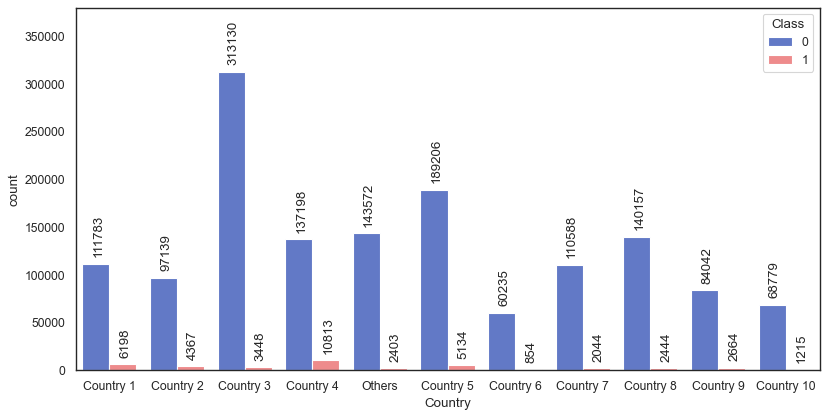
\includegraphics[width=1\textwidth]{figures/evaluation/Image_CountryBarPlot.png}
      \caption[觀察設備所在地之付費玩家與非付費玩家數量長條圖]{觀察設備所在地之付費玩家與非付費玩家數量長條圖\ (\ X軸為設備所在地;Y軸為玩家數量\ )\ }
      \label{fig:eva_CountryBarPlot}
    \end{center}
\end{figure}
\newpage

\begin{figure}[!htb]
    \begin{center}
      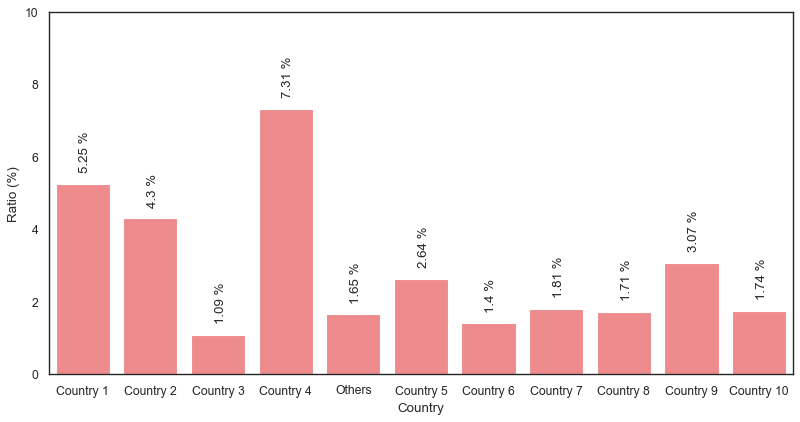
\includegraphics[width=1\textwidth]{figures/evaluation/Image_CountryPayerRatioBarPlot.png}
      \caption[觀察設備所在地之付費玩家比例長條圖]{觀察設備所在地之付費玩家比例長條圖\ (\ X軸為設備所在地;Y軸為付費玩家比例\ )\ }
      \label{fig:eva_CountryPayerRatioBarPlot}
    \end{center}
\end{figure}

利用長條圖觀察在資料集中是否有不合適之資料特徵存在,如圖~\ref{fig:eva_UnreasonableFeatureBarPlot},該圖為GameTypeE 59遊戲之總贏遊戲次數,從圖中可以看出,僅有付費玩家有數值,而非付費玩家則全數皆為0,造成此種現象之原因為因為該款遊戲僅有付費玩家可以遊玩,故將不適合當作資料特徵,予以刪除。

\begin{figure}[!htb]
    \begin{center}
      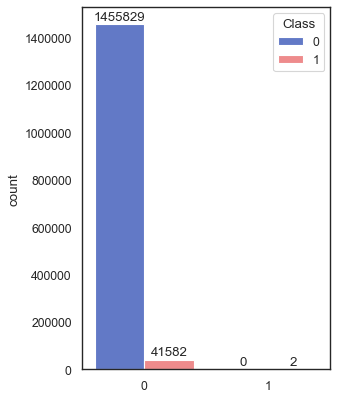
\includegraphics[width=0.4\textwidth]{figures/evaluation/Image_UnreasonableFeatureBarPlot.png}
      \caption[觀察GameTypeE 59號遊戲之總贏遊戲次數長條圖]{觀察GameTypeE 59號遊戲之總贏遊戲次數長條圖\ (\ X軸為總贏遊戲次數;Y軸為玩家數量\ )\ }
      \label{fig:eva_UnreasonableFeatureBarPlot}
    \end{center}
\end{figure}
\newpage

利用散佈圖觀察在資料集中的高資訊量資料特徵,如圖~\ref{fig:eva_ValuableFeatureScatterPlot_GameTypeA} (a) 及圖~\ref{fig:eva_ValuableFeatureScatterPlot_GameTypeA} (b),該圖組為GameTypeA之總贏分與遊戲貨幣A之餘額變化,從兩圖中可以看出,付費玩家與非付費玩家之分佈有明顯差異,推測可以帶給學習模型很好的分類資訊。

\begin{figure}[!htb]
    \centering
    \subfigure[總贏分散佈圖\ (\ X軸為非付費玩家與付費玩家;Y軸為總贏分\ )\ ] {
      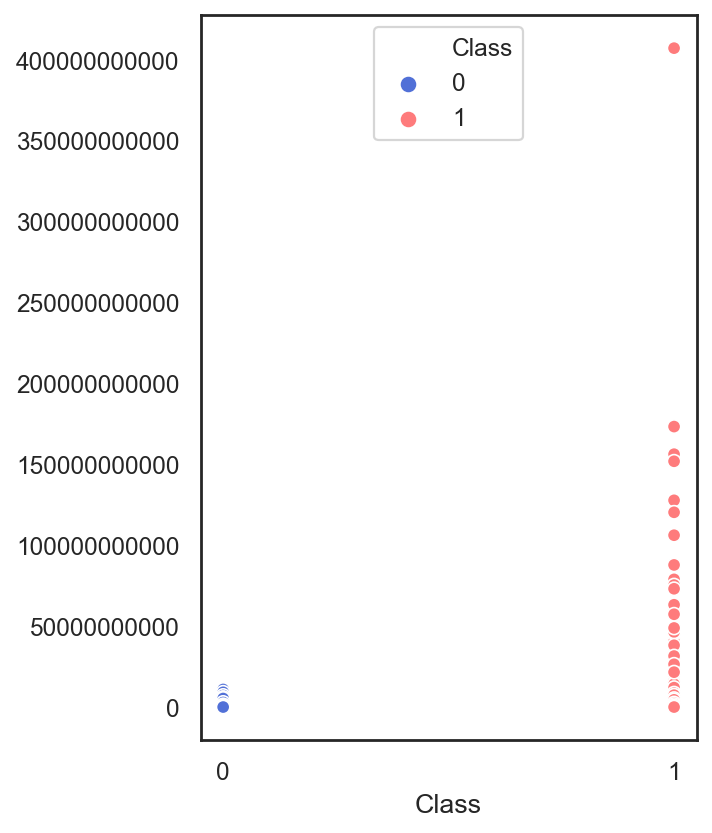
\includegraphics[width=0.45\columnwidth]{figures/evaluation/Image_GameTypeATotalWin.png}
    }
    \subfigure[遊戲貨幣A之餘額變化散佈圖\ (\ X軸為非付費玩家與付費玩家;Y軸為遊戲貨幣A之餘額變化\ )\ ] {
        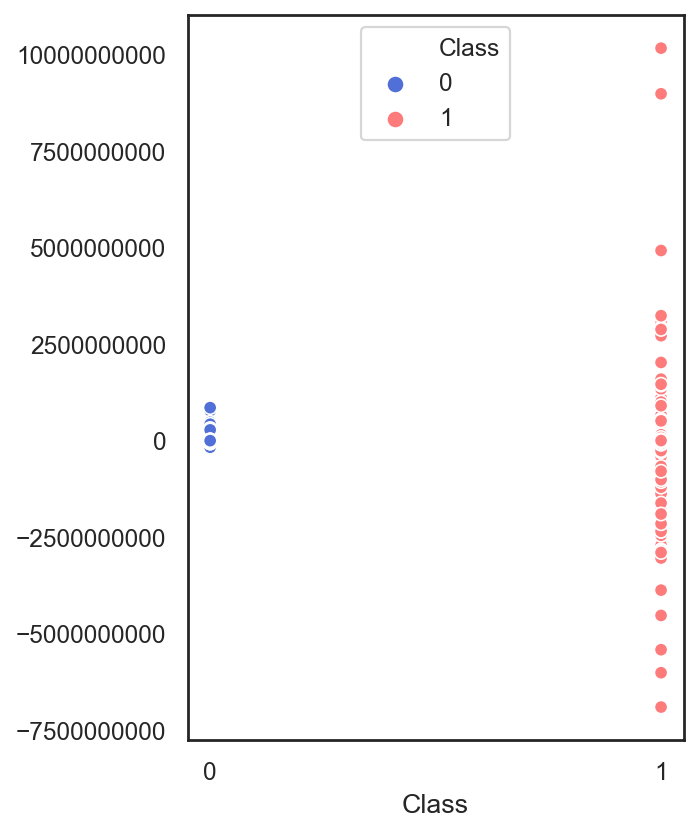
\includegraphics[width=0.45\columnwidth]{figures/evaluation/Image_GameTypeABalanceDiff.png}
    }
    \caption[觀察GameTypeA資料特徵散佈圖]{觀察GameTypeA資料特徵散佈圖}
    \label{fig:eva_ValuableFeatureScatterPlot_GameTypeA}
\end{figure}
\newpage

圖~\ref{fig:eva_ValuableFeatureScatterPlot_GameTypeAWithEntered} (a) 及圖~\ref{fig:eva_ValuableFeatureScatterPlot_GameTypeAWithEntered} (b),該圖組為GameTypeA之遊玩天數與總贏分、遊戲貨幣A之餘額變化,從兩圖中可以看出,隨著遊玩天數的增加,數值的差異性則拉大,推測可以帶給學習模型很好的分類資訊。

\begin{figure}[!htb]
    \centering
    \subfigure[遊玩天數與總贏分散佈圖\ (\ X軸為遊玩天數;Y軸為總贏分\ )\ ] {
      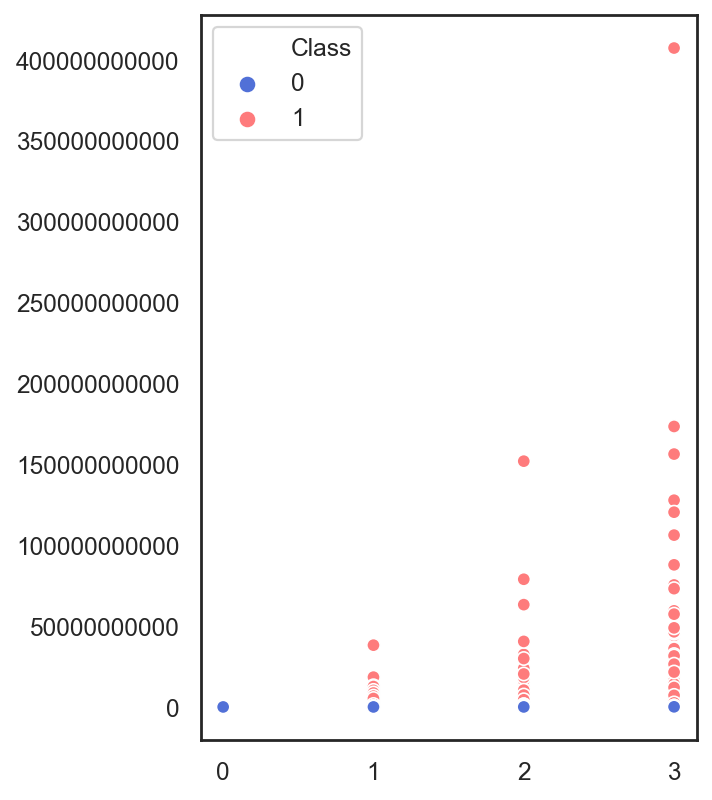
\includegraphics[width=0.45\columnwidth]{figures/evaluation/Image_GameTypeATotalWin&Entered.png}
    }
    \subfigure[遊玩天數與遊戲貨幣A之餘額變化散佈圖\ (\ X軸為遊玩天數;Y軸為遊戲貨幣A之餘額變化\ )\ ] {
        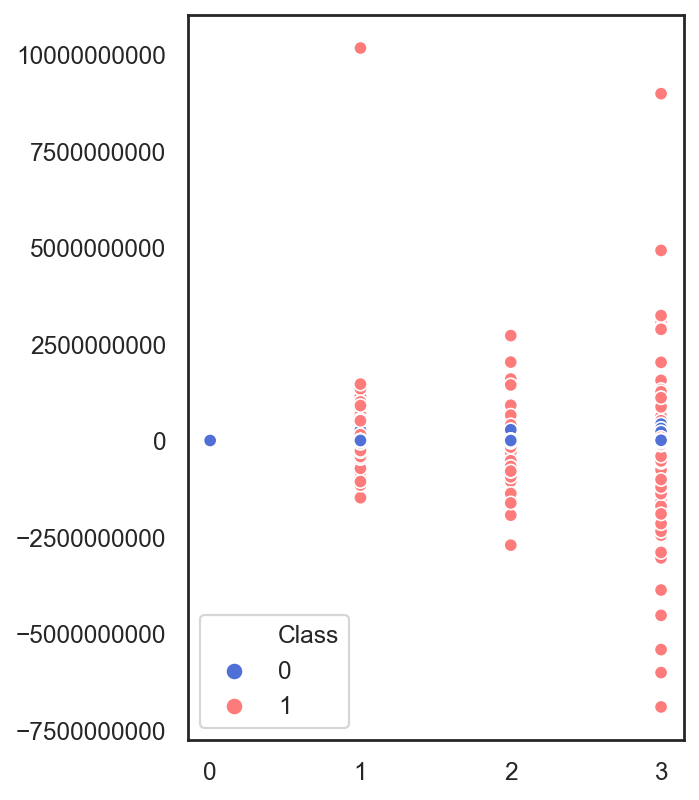
\includegraphics[width=0.45\columnwidth]{figures/evaluation/Image_GameTypeABalanceDiff&Entered.png}
    }
    \caption[觀察GameTypeA資料特徵關聯散佈圖]{觀察GameTypeA資料特徵關聯散佈圖}
    \label{fig:eva_ValuableFeatureScatterPlot_GameTypeAWithEntered}
\end{figure}
\newpage

圖~\ref{fig:eva_ValuableFeatureScatterPlot_GameTypeD65} (a) 及圖~\ref{fig:eva_ValuableFeatureScatterPlot_GameTypeD65} (b),該圖組為GameTypeD 65號遊戲之總贏分與總贏遊戲次數,從兩圖中可以看出,付費玩家與非付費玩家之分佈明顯無差異,推測無法帶給學習模型很好的分類資訊。

\begin{figure}[!htb]
    \centering
    \subfigure[總贏分散佈圖\ (\ X軸為非付費玩家與付費玩家;Y軸為總贏分\ )\ ] {
      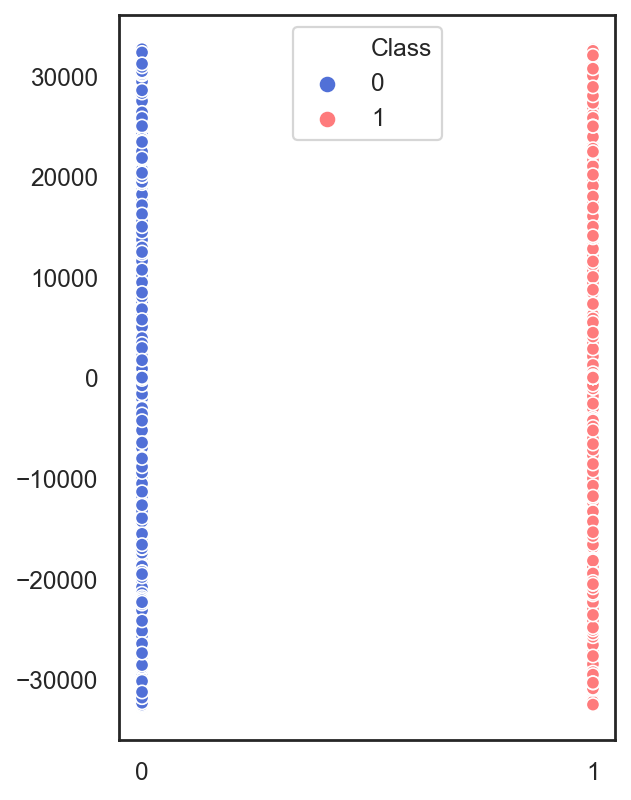
\includegraphics[width=0.45\columnwidth]{figures/evaluation/Image_GameTypeD65TotalWin.png}
    }
    \subfigure[總贏遊戲次數散佈圖\ (\ X軸為非付費玩家與付費玩家;Y軸為總贏遊戲次數\ )\ ] {
        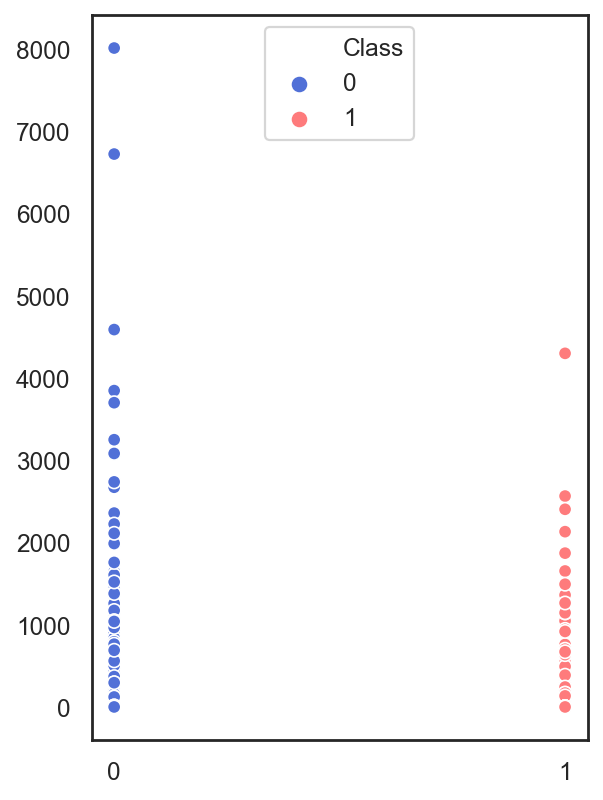
\includegraphics[width=0.45\columnwidth]{figures/evaluation/Image_GameTypeD65TotalWinTimes.png}
    }
    \caption[觀察GameTypeD 65號遊戲資料特徵關聯散佈圖]{觀察GameTypeD 65號遊戲資料特徵關聯散佈圖}
    \label{fig:eva_ValuableFeatureScatterPlot_GameTypeD65}
\end{figure}
\newpage

圖~\ref{fig:eva_ValuableFeatureBarPlot_GameTypeE62TotalWinTimes},該圖為GameTypeE 62號遊戲之總贏遊戲次數,從圖中可以看出,在贏遊戲次數偏低時,非付費玩家佔了大多數,而付費玩家則相對偏少,推測可以帶給學習模型很好的分類資訊。

\begin{figure}[!htb]
    \begin{center}
      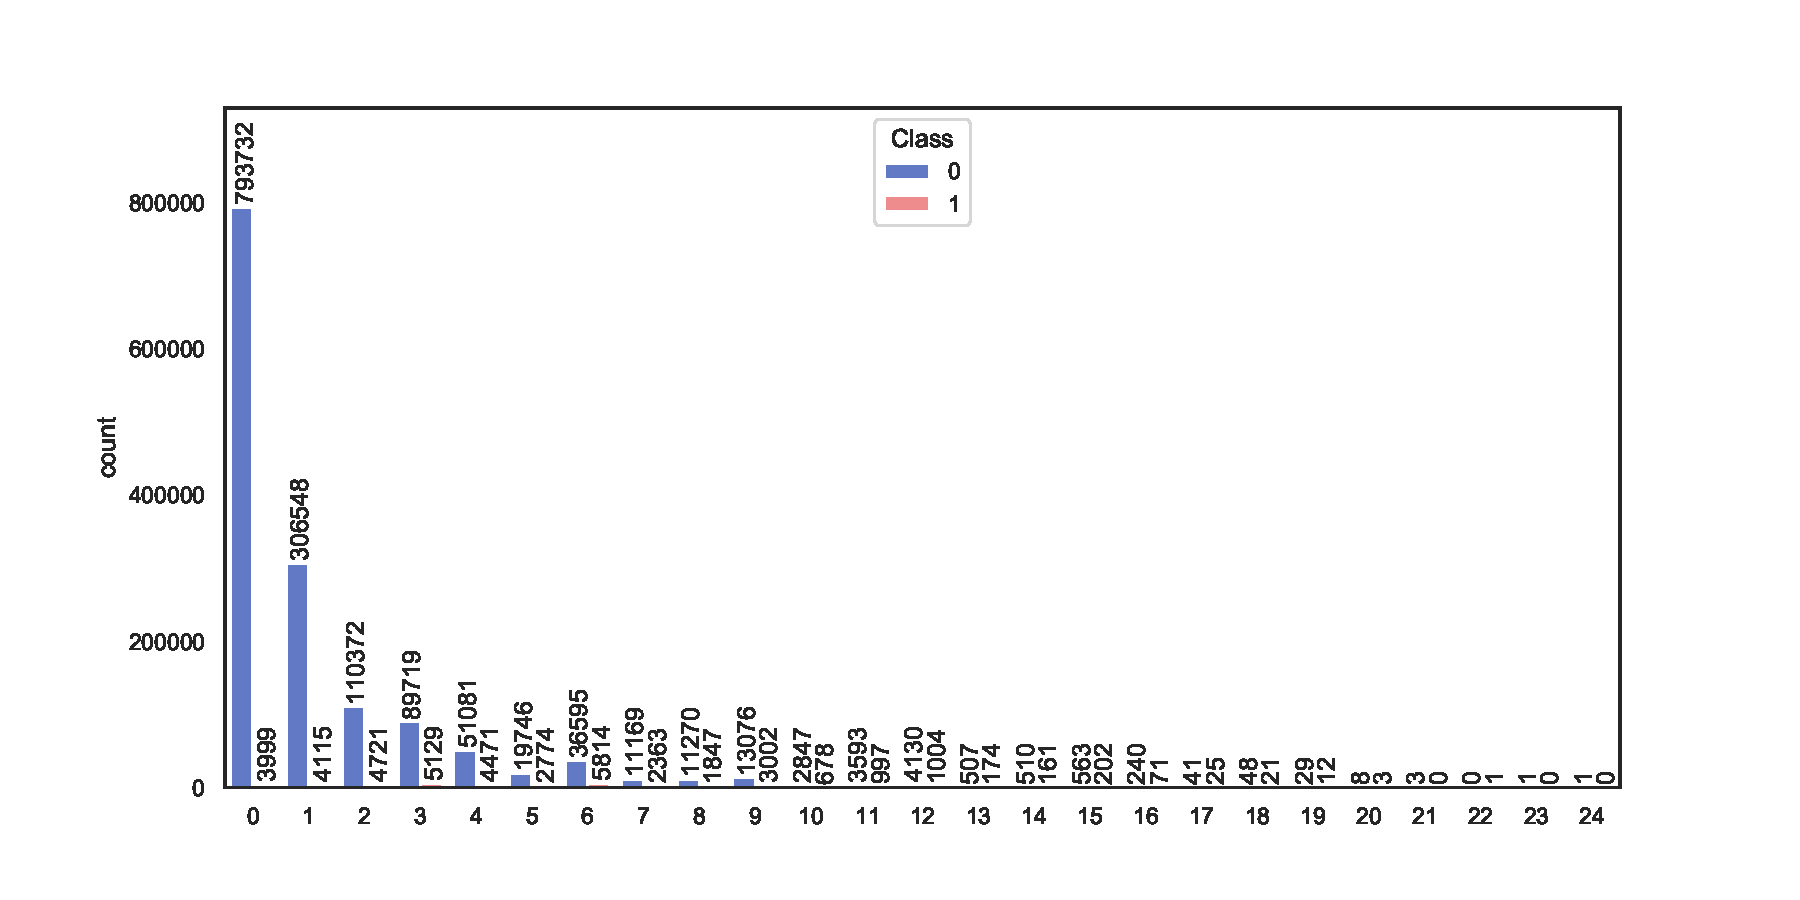
\includegraphics[width=1\textwidth]{figures/evaluation/Image_GameTypeE62TotalWinTimes.pdf}
      \caption[觀察GameTypeE 62號遊戲之總贏遊戲次數長條圖]{觀察GameTypeE 62號遊戲之總贏遊戲次數長條圖\ (\ X軸為總贏遊戲次數;Y軸為玩家數量\ )\ }
      \label{fig:eva_ValuableFeatureBarPlot_GameTypeE62TotalWinTimes}
    \end{center}
\end{figure}

圖~\ref{fig:eva_ValuableFeatureScatterPlot_GameTyeE62TotalCoinAAwarded},該圖為GameTypeE 62號遊戲之獲得遊戲貨幣A之總額,從圖中可以看出,付費玩家資料分佈較廣,而非付費玩家則侷限在10,000左右,推測可以帶給學習模型很好的分類資訊。

\begin{figure}[!htb]
    \begin{center}
      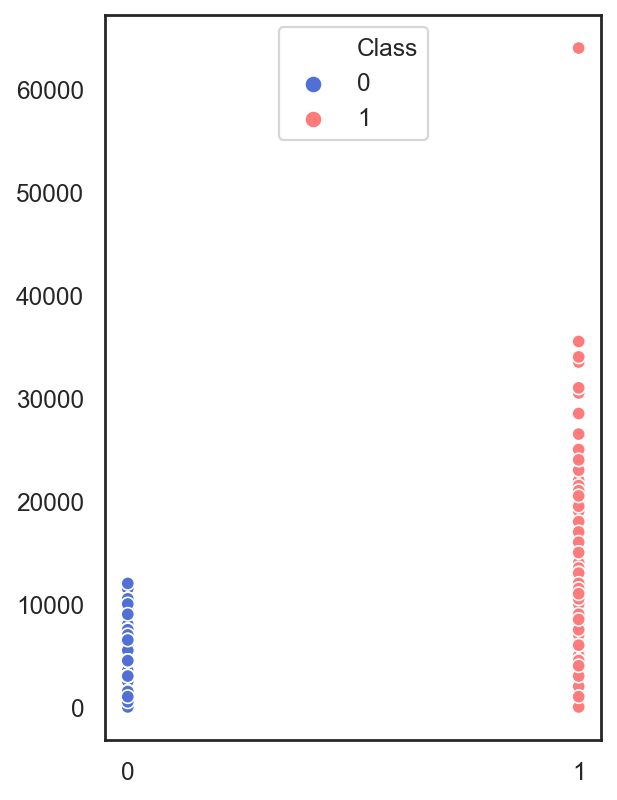
\includegraphics[width=0.4\textwidth]{figures/evaluation/Image_GameTypeE62TotalCoinAAwarded.png}
      \caption[觀察GameTypeE 62號遊戲之獲得遊戲貨幣A之總額散佈圖]{觀察GameTypeE 62號遊戲之獲得遊戲貨幣A之總額散佈圖\ (\ X軸為非付費玩家與付費玩家;Y軸為獲得遊戲貨幣A之總額\ )\ }
      \label{fig:eva_ValuableFeatureScatterPlot_GameTyeE62TotalCoinAAwarded}
    \end{center}
\end{figure}
\newpage

\section{機器學習評估}
\label{sec:MachineLearningEvaluation}

此階段將評估前章 \ref{subsec:SplitDataset}~小節之分割訓練與測試資料集處理、\ref{subsec:ModelSelection}~小節之學習模型選擇與 \ref{subsec:ImbalancedDataHandle}~小節之資料不平衡處理及 \ref{subsec:TuningBestParams}~小節之搜尋最佳參數解處理與 \ref{subsec:CrossValidation}~小節之交叉驗證處理,分別於 \ref{subsec:SplitDatasetEvaluation}~小節\ 分割訓練與測試資料集評估、\ref{subsec:ImbalancedDataHandleEvaluation}~小節\ 資料不平衡處理評估及 \ref{subsec:BestModelEvaluation}~小節\ 最佳模型評估說明。

以下實驗環境將透過\emph{pandas}、\emph{scikit-learn}以及\emph{XGBoost}來進行機器學習之訓練與驗證,並透過\emph{Seaborn}協助呈現驗證結果。
\newpage

\subsection{分割訓練與測試資料集評估}
\label{subsec:SplitDatasetEvaluation}

將資料集依照7:3之比例分割,如圖~\ref{fig:Image_SplitDataset},即為前7週設為訓練集;後3週設為測試集,圖~\ref{fig:eva_NewlyPlayerPerWeek} 為各週之新進玩家數圖,深色底為付費玩家、淺色底為非付費玩家,從圖中可以看出,每週之付費玩家數及非付費玩家數皆大致相等,以週次分割資料集可以保存資料穩定性。

\begin{figure}[!htb]
    \begin{center}
      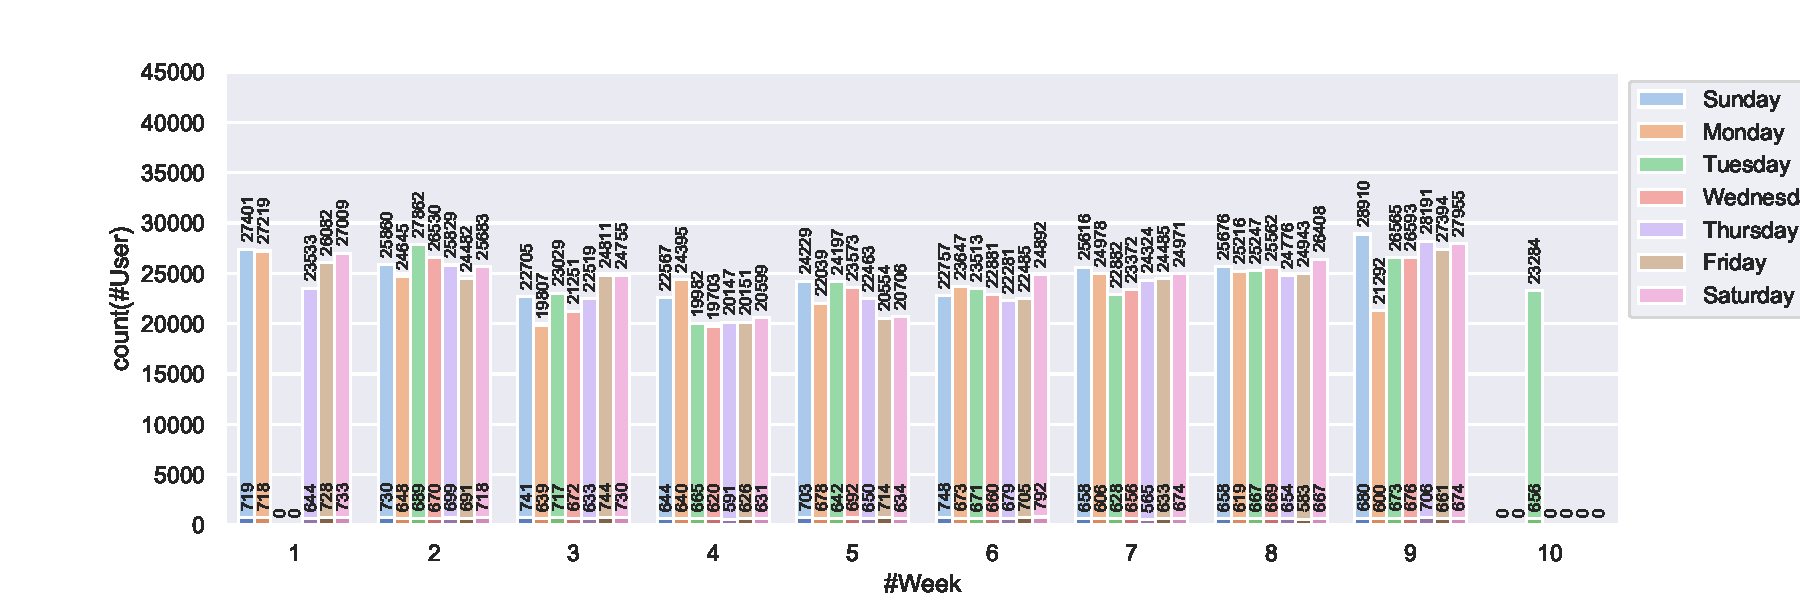
\includegraphics[width=1\textwidth]{figures/evaluation/Image_NewlyPlayerPerWeek.pdf}
      \caption[各週之新進玩家數圖]{各週之新進玩家數圖\ (\ X軸為週次;Y軸為玩家數\ )\ }
      \label{fig:eva_NewlyPlayerPerWeek}
    \end{center}
\end{figure}

表~\ref{tab:NumberOfSplitedPayerAndNonPayer} 為分割完資料集後之付費玩家數與非付費玩家數,訓練資料集與測試資料集之付費玩家與非付費玩家比例皆與原資料集大致相等,分別為33倍與38倍,原資料集為35倍。

\begin{table}[!htb]
	\centering
	\begin{tabular}{|c|r|r|}
	\hline \hline
	\diagbox{資料集}{玩家數} & 付費玩家 & 非付費玩家 \\
    \hline \hline
    訓練集 & 31,741 & 1,077,660 \\
    \hline
    測試集 & 9,843 & 378,169 \\
    \hline \hline
	\end{tabular}
	\caption[訓練與測試資料集玩家數表]{訓練與測試資料集玩家數表}
	\label{tab:NumberOfSplitedPayerAndNonPayer}
\end{table}
\newpage

\subsection{資料不平衡處理評估}
\label{subsec:ImbalancedDataHandleEvaluation}

依照式~\ref{eq:SampleWeightFormula} 計算付費玩家樣本之放大權重,如式~\ref{eq:SampleWeightCalculation},最後將付費玩家之樣本權重放大33倍。以下將進行學習模型之評估,其中將藉由$Confusion\ Matrix$、$Precision$、$Recall$、$True\ Positive\ Rate\ (\ TPR\ )$及$False\ Positive\ Rate\ (\ FPR\ )$來說明評估,計算方式分別如表~\ref{tab:ConfusionMatrix}、式~\ref{eq:PrecisionFormula}、式~\ref{eq:RecallFormula}、式~\ref{eq:TPRFormula} 及式~\ref{eq:FPRFormula}。

\begin{equation}
    \label{eq:SampleWeightCalculation}
    class\ 0 : class\ 1 = 1 : \left \lfloor{\frac{1,077,660}{31,741}}\right \rfloor = 1 : 33
\end{equation}

\begin{table}[!htb]
	\centering
	\begin{tabular}{|c|c|c|}
	\hline
	& True $class\ 1$ & True $class\ 0$ \\
    \hline
    Predicted $class\ 1$ & $True\ Positive\ (\ TP\ )$ & $False\ Positive\ (\ FP\ )$ \\
    \hline
    Predicted $class\ 0$ & $False\ Negative\ (\ FN\ )$ & $True\ Negative\ (\ TN\ )$ \\
    \hline
	\end{tabular}
	\caption[Confusion Matrix]{Confusion Matrix}
	\label{tab:ConfusionMatrix}
\end{table}

\begin{equation}
    \label{eq:PrecisionFormula}
    Precision = \frac{TP}{TP + FP}
\end{equation}

\begin{equation}
    \label{eq:RecallFormula}
    Recall = \frac{TP}{TP + FN}
\end{equation}

\begin{equation}
    \label{eq:TPRFormula}
    True\ Positive\ Rate\ (\ TPR\ ) = \frac{TP}{TP + FN} = Recall
\end{equation}

\begin{equation}
    \label{eq:FPRFormula}
    False\ Positive\ Rate\ (\ FPR\ ) = \frac{FP}{TN + FP}
\end{equation}
\newpage

我們將藉由Receiver Operating Characteristic Curve ( ROC Curve ) 以及Precision-Recall Curve ( PR Curve ) 來觀察學習模型間的$Precision$、$Recall$、\\$True\ Positive\ Rate\ (\ TPR\ )$及$False\ Positive\ Rate\ (\ FPR\ )$,如圖~\ref{fig:eva_ROCCurve} 及圖~\ref{fig:eva_PRCurve}。前者於X軸及Y軸皆以值越大越理想,故曲線越趨近於右上角則越佳;後者於X軸為值越小越理想、Y軸為值越大越理想,故曲線越趨近於左上角則越佳。將再分別利用AUC及AP來衡量兩曲線,皆為計算該曲線面積。

\begin{figure}[!htb]
    \begin{center}
      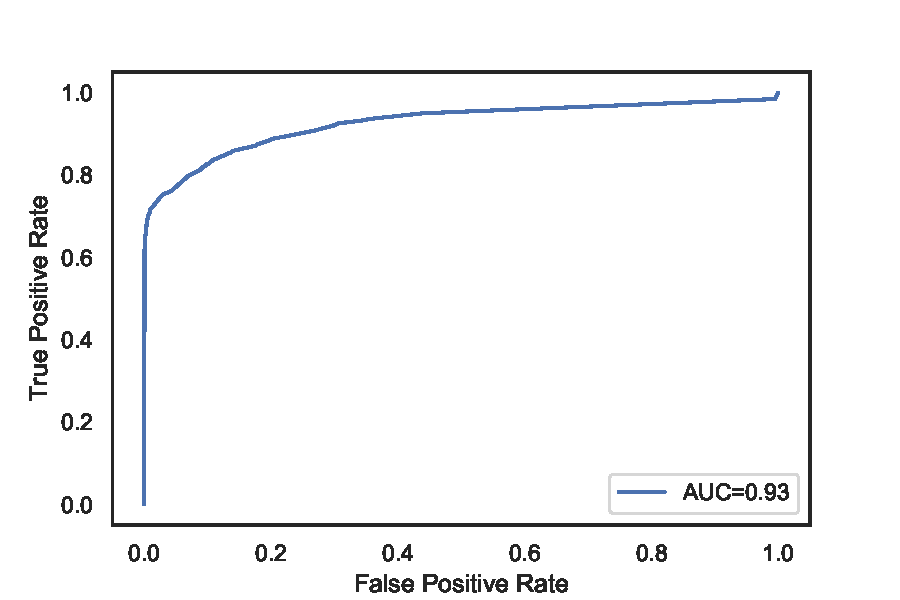
\includegraphics[width=0.7\textwidth]{figures/evaluation/Image_ROCCurve.pdf}
      \caption[ROC Curve示意圖]{ROC Curve示意圖\ (\ X軸為$False\ Positive\ Rate\ (\ FPR\ )$;Y軸為$True\ Positive\ Rate\ (\ TPR\ )$\ ;\ AUC為其曲線面積\ )}
      \label{fig:eva_ROCCurve}
    \end{center}
\end{figure}

\begin{figure}[!htb]
    \begin{center}
      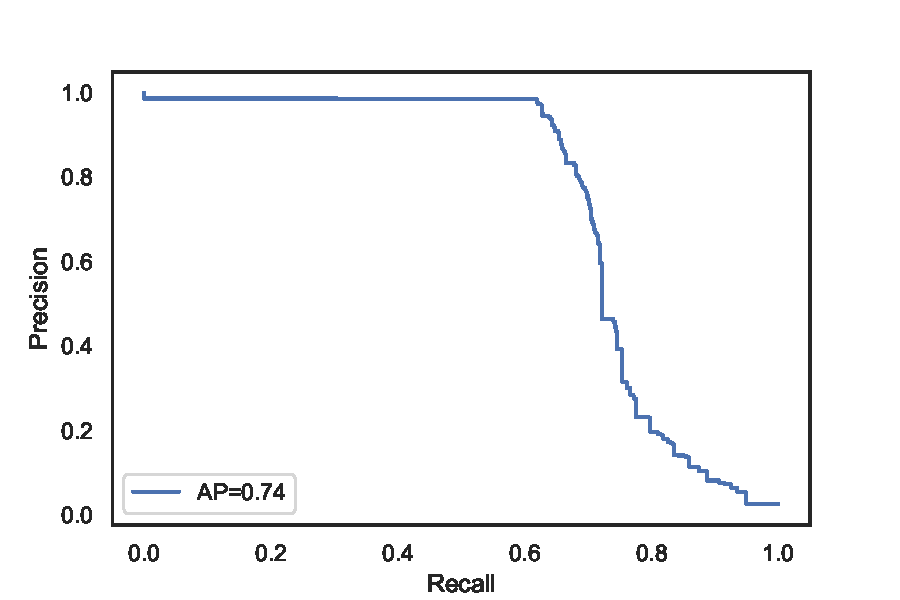
\includegraphics[width=0.7\textwidth]{figures/evaluation/Image_PRCurve.pdf}
      \caption[PR Curve示意圖]{PR Curve示意圖\ (\ X軸為$Recall$;Y軸為$Precision$\ ;\ AP為其曲線面積\ )}
      \label{fig:eva_PRCurve}
    \end{center}
\end{figure}
\newpage

本論文將以評估PR Curve為重,因在不平衡資料集上進行評估時,ROC Curve將無法準確的呈現出學習模型的好壞,常有在ROC Curve上表現良好,但其PR Curve卻不如預期,導致此情況原因為多數群之評估遠大於少數群之評估,故可在ROC Curve上擁有好的數值,卻在PR Curve中表現不佳\cite{davis2006relationship},如圖~\ref{fig:eva_GoodROCBadPR}。

\begin{figure}[!htb]
    \begin{center}
      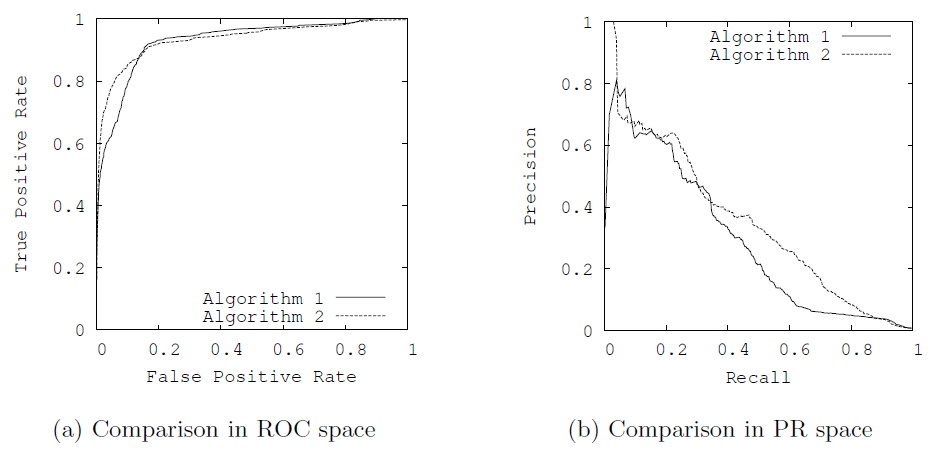
\includegraphics[width=1\textwidth]{figures/evaluation/Image_GoodROCBadPR.png}
      \caption[不平衡資料中ROC Curve失準示意圖]{不平衡資料中ROC Curve失準示意圖\ (\ 此圖取自~\cite{davis2006relationship}\ )}
      \label{fig:eva_GoodROCBadPR}
    \end{center}
\end{figure}
\newpage

圖~\ref{fig:eva_ROCCurveEvaluationImbalancedData} 為三種學習模型之ROC Curve,並比較不平衡資料處理前後之差異,(a)為Decision Tree、(b)為Random Forest、(c)為XGBoost,藍色線為未加入權重值、紅色底為加入權重值,從圖組中可以看出,在付費玩家之樣本權重上進行放大,有助於學習模型之分類,使預設更加準確。AUC最高值於XGBoost加入權重值,為0.95。

\begin{figure}[!htb]
    \centering
    \subfigure[Decision Tree ROC Curve圖] {
      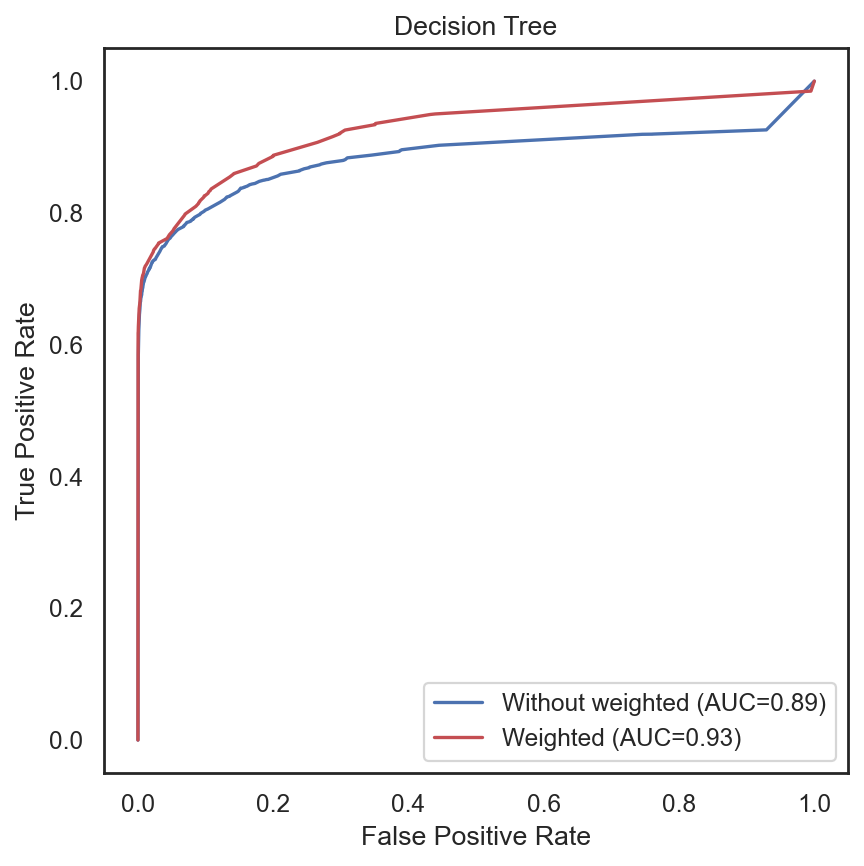
\includegraphics[width=0.47\columnwidth]{figures/evaluation/Image_DTROCCurve.png}
    }
    \subfigure[Random Forest ROC Curve圖] {
        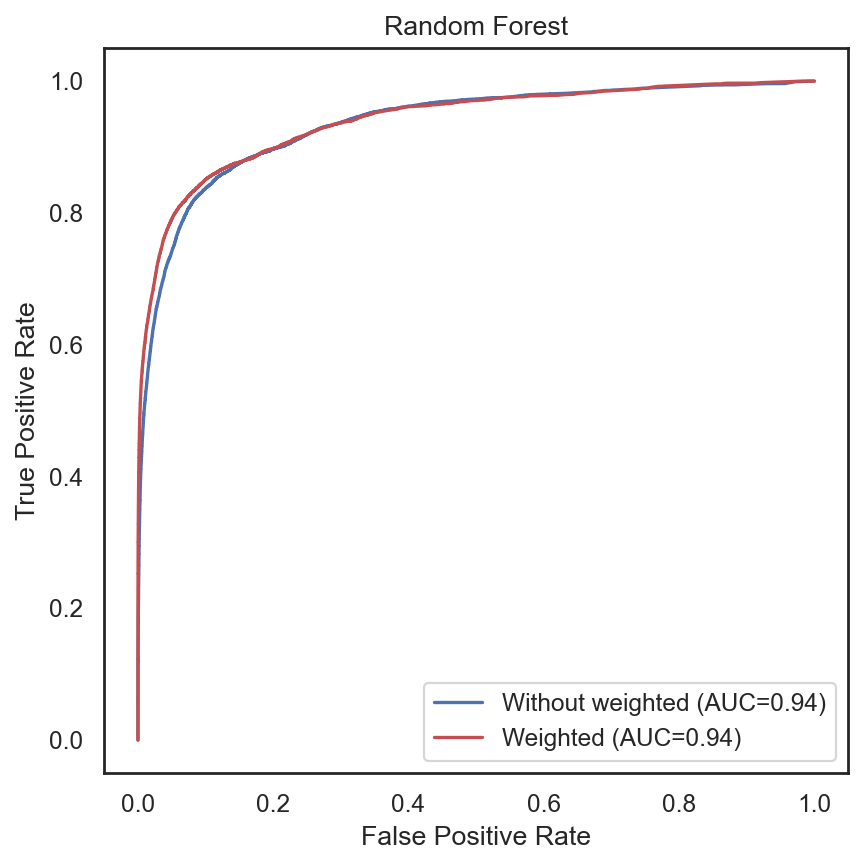
\includegraphics[width=0.47\columnwidth]{figures/evaluation/Image_RFROCCurve.png}
    }
    \subfigure[XGBoost ROC Curve圖] {
        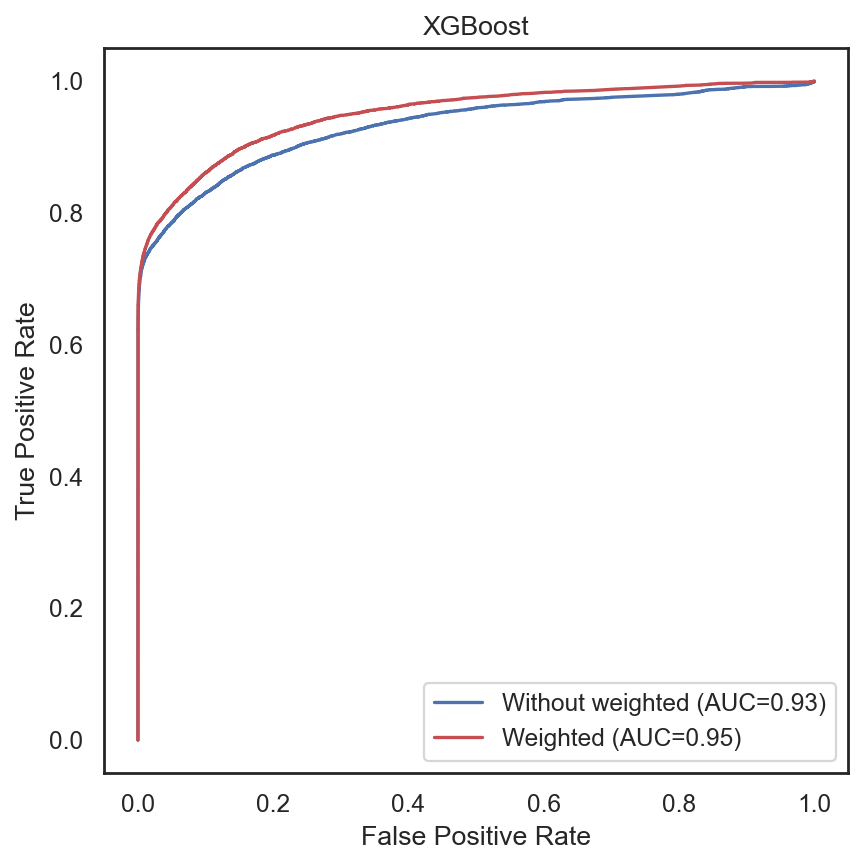
\includegraphics[width=0.47\columnwidth]{figures/evaluation/Image_XGBROCCurve.png}
    }
    \caption[不平衡資料處理前後比較之ROC Curve圖]{不平衡資料處理前後比較之ROC Curve圖\ (\ X軸為$False\ Positive\ Rate (\ FPR\ )$;Y軸為$True\ Positive\ Rate (\ TPR\ )$\ )}
    \label{fig:eva_ROCCurveEvaluationImbalancedData}
\end{figure}
\newpage

圖~\ref{fig:eva_PRCurveEvaluationImbalancedData} 為三種學習模型之PR Curve,並比較不平衡資料處理前後之差異,(a)為Decision Tree、(b)為Random Forest、(c)為XGBoost,藍色線為未加入權重值、紅色底為加入權重值,從圖組中可以看出,在付費玩家之樣本權重上進行放大,有助於學習模型之分類,使預設更加準確。AP最高值於XGBoost加入權重值,為0.79。

\begin{figure}[!htb]
    \centering
    \subfigure[Decision Tree PR Curve圖] {
      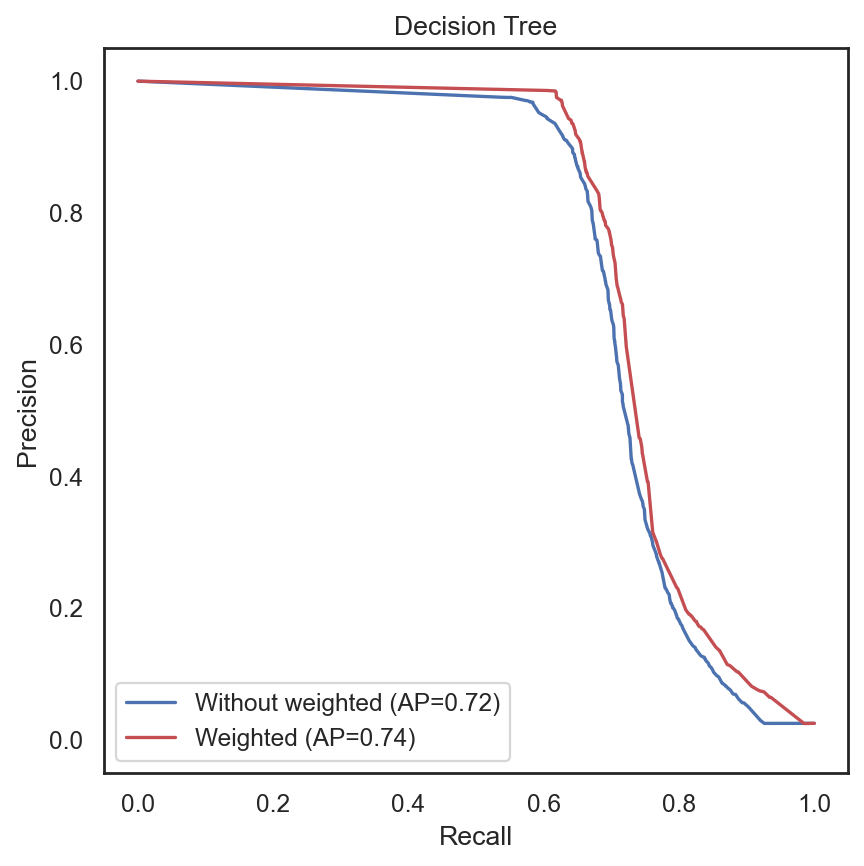
\includegraphics[width=0.47\columnwidth]{figures/evaluation/Image_DTPRCurve.png}
    }
    \subfigure[Random Forest PR Curve圖] {
        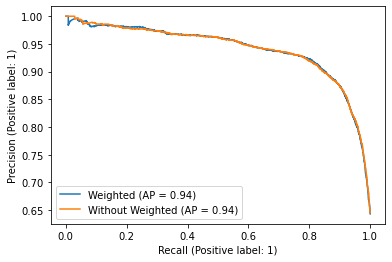
\includegraphics[width=0.47\columnwidth]{figures/evaluation/Image_RFPRCurve.png}
    }
    \subfigure[XGBoost PR Curve圖] {
        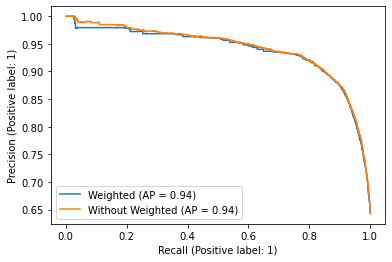
\includegraphics[width=0.47\columnwidth]{figures/evaluation/Image_XGBPRCurve.png}
    }
    \caption[不平衡資料處理前後比較之PR Curve圖]{不平衡資料處理前後比較之PR Curve圖\ (\ X軸為$Recall$;Y軸為$Precision$\ )}
    \label{fig:eva_PRCurveEvaluationImbalancedData}
\end{figure}

上述兩種評估方式皆為在加入權重值後,改進了學習模型的訓練,使其不受於資料不平衡之影響,且適用於三種學習模型。
\newpage

\subsection{最佳模型評估}
\label{subsec:BestModelEvaluation}

利用Repeated Stratified Cross Validation來調教出最佳模型,我們將採用Reapted 2次及5-Fold Cross Validation,最後使用測試資料集進行評估驗證,其中包含付費玩家 ( $class\ 1$ ) 9,843位及非付費玩家 ( $class\ 0$ ) 378,169位,驗證結果如表~\ref{tab:BestModelEvaluation},從表中可以看出,XGBoost的$Weighted\ F_{beta} - Score$為三者最高,預測能力最佳。

\begin{table}[!htb]
    \centering
        \begin{tabular}{|c|r|r|r|r|}
            \hline \hline
            \multirow{2}*{\diagbox{學習模型}{評估}} & $precision^+$ & $recall^+$ & ${F_{beta}}^+$ & \multirow{2}*{$Weighted\ F_{beta}$} \\
            \cline{2-4}
            & $precision^-$ & $recall^-$ & ${F_{beta}}^-$ & \\
            \hline \hline
            \multirow{2}*{Decision Tree} & 0.700 & 0.726 & 0.726 & \multirow{2}*{0.985} \\
            \cline{2-4}
            & 0.993 & 0.992 & 0.992 & \\
            \hline
            \multirow{2}*{Random Forest} & 0.840 & 0.678 & 0.678 & \multirow{2}*{0.989} \\
            \cline{2-4}
            & 0.992 & 0.997 & 0.997 & \\
            \hline
            \multirow{2}*{XGBoost} & 0.965 & 0.722 & 0.723 & \multirow{2}*{0.992} \\
            \cline{2-4}
            & 0.993 & 0.999 & 0.999 & \\
            \hline
            \multicolumn{5}{|l|}{$+$:以正例(付費玩家 $class\ 1$ )為評估對象進行計算} \\
            \multicolumn{5}{|l|}{$-$:以反例(非付費玩家 $class\ 0$ )為評估對象進行計算} \\
            \hline \hline
        \end{tabular}
    \caption[最佳模型評估表]{最佳模型評估表}
    \label{tab:BestModelEvaluation}
\end{table}

圖~\ref{fig:eva_ModelsROCCurve} 及圖~\ref{fig:eva_ModelsPRCurve} 為三種學習模型之ROC Curve及PR Curve比較圖,並且都為加入權重值之結果,從圖組中可以看出,皆為XGBoost擁有最好的結果,綜合上述得到的實驗結果,我們認為XGBoost非常適用於遊戲領域巨量資料預測分類上,因其Boosting方式建樹,強化修正於分類錯誤樣本,有效的提升學習模型預測之準確度,並採用Gradient Descent來加速學習模型之收斂,減少建樹時間成本。

另外,此處實驗之Random Forest遭遇了前述所提到ROC Curve表現佳,卻在PR Curve表現差的問題,甚至評估結果差於基礎學習模型Decision Tree,有可能是因學習模型有過擬合 ( Overfitting ) 的情形發生,所導致PR Curve表現不佳。
\newpage

\begin{figure}[!htb]
    \begin{center}
      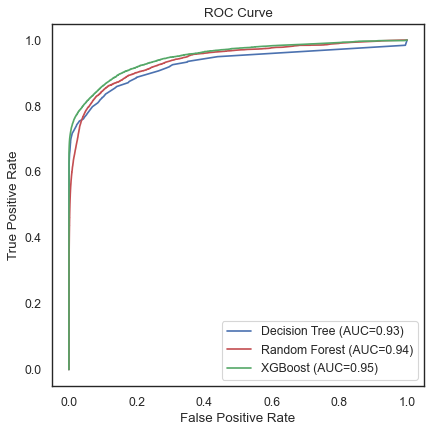
\includegraphics[width=0.6\textwidth]{figures/evaluation/Image_ModelsROCCurve.png}
      \caption[三種學習模型之ROC Curve比較圖]{三種學習模型之ROC Curve比較圖}
      \label{fig:eva_ModelsROCCurve}
    \end{center}
\end{figure}

\begin{figure}[!htb]
    \begin{center}
      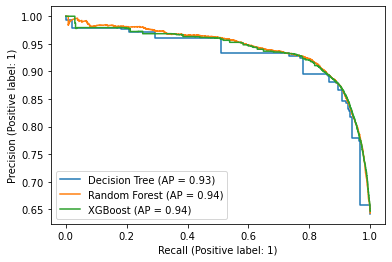
\includegraphics[width=0.6\textwidth]{figures/evaluation/Image_ModelsPRCurve.png}
      \caption[三種學習模型之PR Curve比較圖]{三種學習模型之PR Curve比較圖}
      \label{fig:eva_ModelsPRCurve}
    \end{center}
\end{figure}
\newpage

表~\ref{tab:BestModelParams} 為三種學習模型之最佳參數解,參數搜尋範圍如表~\ref{tab:ParamsSearchRange},Decision Tree因其為單樹結構,相較之下需要生成更深的樹;而Random Forest及XGBoost則因其為多樹結構,希望能以廣度發展,而非深度,相較之下需要生成更多的樹。

\begin{table}[!htb]
    \centering
        \begin{tabular}{clll}
            \hline \hline
            學習模型 & Decision Tree & Random Forest & XGBoost \\
            \hline \hline
            \multirow{4}*{參數調教} & max\char`_depth=13 & n\char`_estimators=55 & n\char`_estimators=55 \\
            & min\char`_samples\char`_split=2 & max\char`_depth=13 & max\char`_depth=10 \\
            & min\char`_samples\char`_leaf=5 & min\char`_samples\char`_split=2 & \\
            && min\char`_samples\char`_leaf=5 & \\
            \hline \hline
        \end{tabular}
    \caption[最佳模型參數解表]{最佳模型參數解表}
    \label{tab:BestModelParams}
\end{table}

\begin{table}[!htb]
    \centering
        \begin{tabular}{cl}
            \hline \hline
            參數名 & 搜尋範圍 \\
            \hline \hline
            n\char`_estimators & 20, 25, 30, 35, 40, 45, 50, 55, 60 \\
            \hline
            max\char`_depth & 1, 2, 3, 4, 5, 6, 7, 8, 9, 10, 11, 12, 13, 14, 15 \\
            \hline
            min\char`_samples\char`_split & 2, 4, 6, 8, 10 \\
            \hline
            min\char`_samples\char`_leaf & 1, 5, 10, 15, 20 \\
            \hline \hline
        \end{tabular}
    \caption[參數搜尋範圍表]{參數搜尋範圍表}
    \label{tab:ParamsSearchRange}
\end{table}
\newpage

\section{預測結果分析評估}
\label{sec:PredictionResultAnalysisEvaluation}

此階段將評估前章 \ref{subsec:FeatureImportanceAnalysis}~小節之資料特徵重要性分析處理,於 \ref{subsec:FeatureImportanceEvaluation}~小節 資料特徵重要性評估說明。

\subsection{資料特徵重要性評估}
\label{subsec:FeatureImportanceEvaluation}

將利用式~\ref{eq:GiniImportanceFormula}、式~\ref{eq:SingleTreeFeatureImportanceFormula} 及式~\ref{eq:ModelFeatureImportanceFormula} 計算之各資料特徵於各模型之資料特徵重要性 ( $Feature\ Importance$, $fi$ ) ,如圖~\ref{fig:eva_DTFeatureImportances}、圖~\ref{fig:eva_RFFeatureImportances} 及圖~\ref{fig:eva_XGBFeatureImportances},分別為Decision Tree、Random Forest及XGBoost之資料特徵重要性比較圖。

\begin{figure}[!htb]
    \begin{center}
      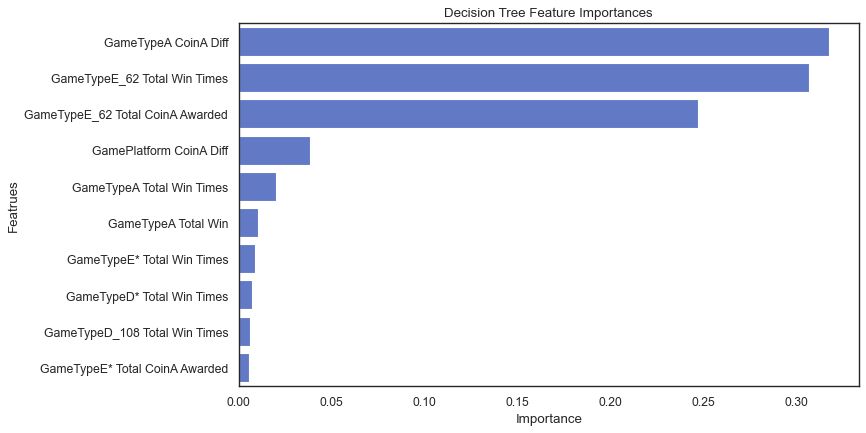
\includegraphics[width=1\textwidth]{figures/evaluation/Image_DTFeatureImportances.png}
      \caption[Decision Tree資料特徵重要性比較圖]{Decision Tree資料特徵重要性比較圖}
      \label{fig:eva_DTFeatureImportances}
    \end{center}
\end{figure}
\newpage

\begin{figure}[!htb]
    \begin{center}
      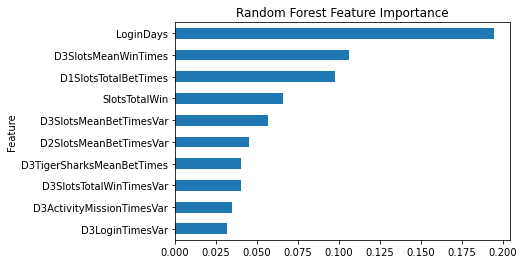
\includegraphics[width=1\textwidth]{figures/evaluation/Image_RFFeatureImportances.png}
      \caption[Random Forest資料特徵重要性比較圖]{Random Forest資料特徵重要性比較圖}
      \label{fig:eva_RFFeatureImportances}
    \end{center}
\end{figure}

\begin{figure}[!htb]
    \begin{center}
      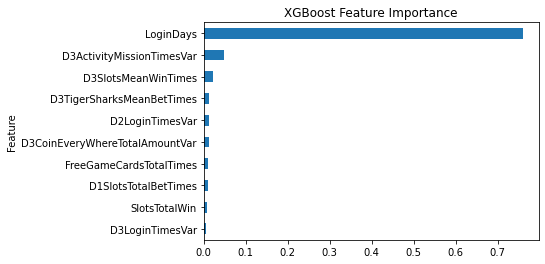
\includegraphics[width=1\textwidth]{figures/evaluation/Image_XGBFeatureImportances.png}
      \caption[XGBoost資料特徵重要性比較圖]{XGBoost資料特徵重要性比較圖}
      \label{fig:eva_XGBFeatureImportances}
    \end{center}
\end{figure}
\newpage

從三圖中可以看出,GameTypeE 62號遊戲的獲得遊戲貨幣A之總額以及總贏遊戲次數皆在三種學習模型的前四名,可以說明此款遊戲在於玩家獲得獎勵及贏得遊戲時,對於其付費意願有明顯提升;GameTypeA的遊戲貨幣A之餘額變化以及總贏分皆在前十名,可以說明此款遊戲在於玩家遊玩遊戲時的體驗起伏(無論輸或贏)及贏取分數時,對於其付費意願有明顯提升。

上述所提到的資料特徵皆在 \ref{subsubsec:ValuableFeatures}~小節中有進行推測該類資料特徵將有助於學習模型訓練,顯示先對資料進行分析,對於學習模型之解釋以及後續之利用是有相當程度上的幫助,可以透過探索性資料分析,在資料集應用於機器學習前,即先對資料進行探索,找出資料之問題或是高資訊量的資料特徵,進而增進學習模型的成效或是加強資料特徵的轉化。

另外,三種學習模型之前十名資料特徵皆為數值型的資料特徵,而無類別型資料特徵,因其資料特徵重要性之評估以計算$Gini\ Importance$為主,數值型將會比類別型來得更為顯著,未來將可在計算重要性分析中,對於不同類型的資料特徵加入權重值,使得類別型的資料特徵能夠突出,讓整體分析更加準確。
\newpage